\cotefile{141}
\scanpage{15}
\figure{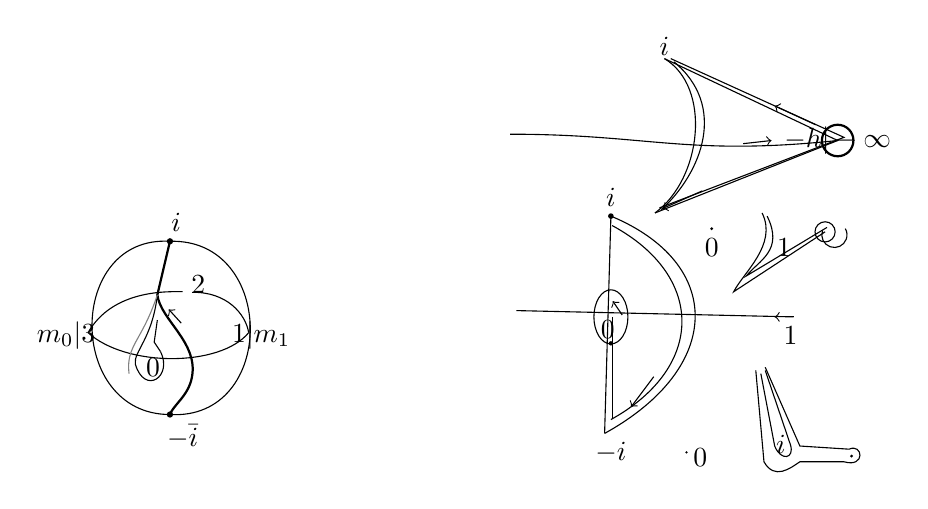
\begin{tikzpicture}[x=.8cm,y=.8cm]
\draw (1.8,3.65)..controls(.15,3.75)and(.15,.9)..(1.8,.9)..controls(3.5,.8)and(3.5,3.7)..(1.8,3.65);
\draw (.5,2.2)..controls(1.1,1.65)and(2.6,1.65)..(3.05,2.2);
\draw (.5,2.2)..controls(.9,2.9)and(1.8,2.85)..(2.0,2.85);
\draw (2.15,2.84)..controls(2.7,2.85)and(3,2.5)..(3.05,2.2);
\draw[thick] (1.8,3.65)--(1.6,2.8)..controls(1.65,2.4)and(2.25,2.05)..(2.15,1.5)..controls(2.1,1.2)and(1.85,1.05)..(1.8,.9);
\draw (1.6,2.8)..controls(1.52,2.1)and(1.22,1.9)..(1.25,1.7)..controls(1.4,1.2)and(1.85,1.5)..(1.65,1.9);
\draw (1.6,2.4)--(1.55,2.05)--(1.65,1.9);
\draw[gray] (1.6,2.8)..controls(1.35,2.05)and(1.1,2)..(1.15,1.55);
\fill (1.8,3.65) circle(.05);\fill (1.8,.9) circle(.05);
\node at (1.9,3.95) {$i$};\node at (2,.55) {$-\bar i$};
\node at (.15,2.15) {$\unsure{m_0|3}$};\node at (3.25,2.15) {$\unsure{1|m_1}$};
\node at (2.25,2.96) {$2$};\node at (1.53,1.65) {$0$};\draw[->] (1.98,2.35)--(1.78,2.57);
\draw (9.65,6.55)--(12.4,5.25)--(9.5,4.1);
\draw (9.75,6.55)--(12.5,5.3)--(9.57,4.18);
\draw (9.65,6.55)..controls(10.4,6.1)and(10.25,4.65)..(9.5,4.1);
\draw (9.8,6.5)..controls(10.65,5.8)and(10.25,4.75)..(9.6,4.15);
\draw[->] (12.05,5.5)--(11.4,5.8);\draw[->] (10.25,4.45)--(9.62,4.17);
\draw (7.2,5.35)..controls(9.4,5.35)and(10,5)..(12.4,5.25);
\draw[->] (10.9,5.2)--(11.35,5.25);
\draw[thick] (12.4,5.25) circle(.25);\node at (12.4,5.25) {$\unsure{-h|-\infty}$};
\node at (9.65,6.75) {$\unsure{i}$};
\draw (8.8,4.05)--(8.7,.6);
\draw (8.8,4.05)..controls(10.6,3.3)and(10.6,1.65)..(8.7,.6);
\draw (8.82,3.9)..controls(10.3,3.1)and(10.3,1.65)..(8.8,.82);
\draw (8.82,2.45)--(8.82,.85);\draw[->] (9.48,1.5)--(9.12,1.02);
\draw (7.3,2.55)--(11.7,2.45);\draw[->] (11.7,2.45)--(11.4,2.45);
\draw (8.8,2.45) ellipse (.27 and .43);
\draw[->] (8.98,2.48)--(8.83,2.7);\node at (8.75,2.25) {$0$};
\node at (8.8,4.35) {$i$};\node at (8.8,.3) {$-i$};\node at (11.65,2.15) {$1$};
\fill (8.8,4.05) circle(.045);\fill (8.8,2.03) circle(.035);
\node at (10.4,3.55) {$0$};\fill (10.4,3.85) circle(.025);
\draw (11.2,4.1)..controls(11.45,3.6)and(10.9,3.15)..(10.75,2.85)--(12.2,3.8);
\draw (11.28,4.05)..controls(11.55,3.5)and(11.15,3.35)..(10.95,3.1)--(12.23,3.87);
\draw (12.2,3.8) circle(.16);\draw (12.16,3.82) arc[start angle=160,end angle=390,radius=.2];
\node at (11.55,3.55) {$1$};
\draw (11.1,1.6)--(11.23,.15)..controls(11.4,-.15)and(11.65,.05)..(11.8,.15)--(12.5,.15)..controls(12.85,.05)and(12.8,.45)..(12.58,.35)--(11.8,.4)--(11.25,1.65);
\draw (11.18,1.55)--(11.4,.4)..controls(11.5,.15)and(11.72,.2)..(11.65,.42)--(11.25,1.6);
\node at (11.5,.42) {$i$};\fill (12.62,.24) circle(.025);
\fill (10,.3) circle(.02);\node at (10.22,.21) {$0$};
\end{tikzpicture}}

\[
\pi\qquad\lambda_0\ \lambda_1\ \lambda_2\ \lambda_3\qquad\varepsilon
\]
\deleted{\[
\lambda_0\lambda_1\lambda_2\lambda_3=1
\]}
% Second pass: a horizontal rule is drawn between the struck line above and this line; this line is not struck.
\[
\lambda_3\lambda_2\lambda_1\lambda_0=1
\]
\[
\varepsilon^2=1\qquad
\begin{cases}\varepsilon\lambda_0\varepsilon^{-1}=\lambda_0^{-1}\\
\varepsilon\lambda_1\varepsilon^{-1}=\lambda_1^{-1}
\end{cases}
\qquad\varepsilon\lambda_i\varepsilon^{-1}
\]
\[
\operatorname{Hom}(i,-i)
\]
\diagram{\begin{tikzcd}[ampersand replacement=\&,column sep=large,row sep=small]
\operatorname{Hom}(-i,-i)\arrow[d,phantom,"\wr"]\&\operatorname{Hom}(i,i)\arrow[d,phantom,"\wr"]\\
\pi\&\pi
\end{tikzcd}}
\[
\deleted{\unsure{\ell\circ\bar\ell^{-1}|\ell\circ\bar\ell}}\qquad\lambda_1^{-1}\lambda_2^{-1}\lambda_1
\]
\diagram{\begin{tikzcd}[ampersand replacement=\&,column sep=large]
i\arrow[r,"\varepsilon^{-1}"]\&\bar i\&\bar i\arrow[r,"\overset{\longleftarrow}{\lambda_i}"]\&\bar i\&\bar i\arrow[r,"\varepsilon"]\&i
\end{tikzcd}}
\[
\varepsilon\circ\bar\lambda_i\circ\varepsilon^{-1}.
\]

\figure{\begin{tikzpicture}\fill (0,0) circle(.025);\end{tikzpicture}}
\diagram{\begin{tikzcd}[ampersand replacement=\&,row sep=small]
X\arrow[d,phantom,"\rotatebox{90}{$\in$}"]\&\Gamma\\a\&
\end{tikzcd}}
\[
(\gamma\in\Gamma,\ell\in\operatorname{Hom}(\gamma a,\deleted{\gamma}b))
\]
\[
(\gamma'\in\Gamma,\ell'\in\operatorname{Hom}(\gamma'b,\deleted{\gamma'}c))
\]
\[
\pi_1(X,\Gamma;a)\longrightarrow\Gamma
\]

\diagram{\begin{tikzcd}[ampersand replacement=\&,column sep=large,row sep=large]
\gamma a\arrow[r,"\ell"]\&\deleted{\gamma}b\&\deleted{\gamma'a\ \gamma'\ell}:\\
\&\gamma'b\arrow[r,"\ell'"]\&\deleted{\gamma'}c
\end{tikzcd}}
\deleted{\diagram{\begin{tikzcd}[ampersand replacement=\&,column sep=large]
\gamma b\arrow[r,"\gamma\ell'"]\&\gamma\gamma'c
\end{tikzcd}}}

\diagram{\begin{tikzcd}[ampersand replacement=\&,column sep=large]
\gamma'\gamma a\arrow[r,"\gamma'(\ell)"]\&\gamma'b\arrow[r,"\ell'"]\&c
\end{tikzcd}}

\diagram{\begin{tikzcd}[ampersand replacement=\&,column sep=large]
a\arrow[r,dash,"(\gamma\ell')\circ\ell"]\&\gamma\gamma'c
\end{tikzcd}}
\[
(\gamma\gamma',(\gamma\ell')\circ\ell)
\]

\figure{\begin{tikzpicture}
\draw (0,.5)--(-.12,-2.8);
\node at (.7,.2) {$\gamma a$};\fill (1.75,.2) circle(.03);
\node at (.7,-.6) {$-\gamma'a$};\draw (1.35,-.6)--(1.8,-.6);\fill (2.05,-.6) circle(.03);
\end{tikzpicture}}

\[
(\gamma',\ell')\bigl(\gamma^{\deleted{\unsure{\prime}}},\ell^{\deleted{\unsure{\prime}}}\bigr)
=\Bigl(\gamma'\gamma^{\deleted{\unsure{\prime}}},
\deleted{(\gamma\ell')\circ\ell}\inserted{\ell'\circ\gamma'(\ell)}\Bigr)
\]
\figure{\begin{tikzpicture}\draw[thick] (0,0)--(.22,0);\end{tikzpicture}}

\mspage{14}
\scanpage{16}
\diagram{\begin{tikzcd}[ampersand replacement=\&,column sep=large]
\operatorname{Ens}(\pi)\arrow[r,"F_X","{}_{\pi'}X_\pi"']\&\operatorname{Ens}(\pi')\arrow[r,"F_Y","{}_{\pi''}Y_{\pi'}"']\&\operatorname{Ens}(\pi'')
%
\end{tikzcd}}
\[
F_Y\circ F_X=F_{Y\wedge_{\pi'}X}
\]
\figure{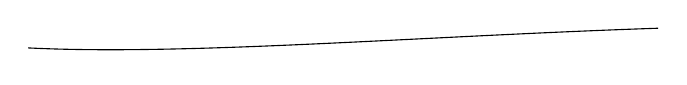
\begin{tikzpicture}\draw (0,0)..controls(2,-.1)and(5,.15)..(8,.25);\end{tikzpicture}}

${}_{\pi'}X_\pi$ bitorseur; classifier à isom près ?

\[
\pi'\xrightarrow{\sim}{}^X\pi
\overset{\substack{\text{non can.}\\\text{mais can. dans }\operatorname{Isomext}({}^X\pi,\pi)}}{\simeq}\pi
\]

Donc $X$ définit $\operatorname{Isomext}(\pi',\pi)$

\deleted{\unsure{Cl d'i.|Classes} de bit $(\pi',\pi)$}
\[
\pi_0\bigl(\underline{\operatorname{Bit}}(\pi',\pi)\bigr)
\xrightarrow{\sim}\operatorname{Isomext}(\pi',\pi)
\]

\diagram{\begin{tikzcd}[ampersand replacement=\&,column sep=large,row sep=huge]
\pi_0\bigl(\underline{\operatorname{Bit\,pt}}(\pi',\pi)\bigr)\arrow[r,phantom,"\simeq"]\arrow[d]\&\operatorname{Isom}(\pi',\pi)\arrow[dl,"\begin{gathered}\text{surj.}\\\text{pass. au quot}\\\text{par }\operatorname{Int}(\pi)\end{gathered}"]\\
\pi_0\bigl(\underline{\operatorname{Bit}}(\pi',\pi)\bigr)\simeq\operatorname{Isom}(\pi',\pi)/\operatorname{Int}(\pi)=\operatorname{Isomext}(\pi',\pi)\&
\end{tikzcd}}

\figure{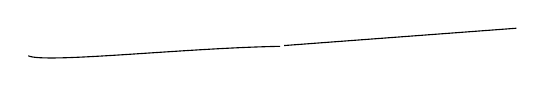
\begin{tikzpicture}\draw (0,0)..controls(.2,-.1)and(2,.1)..(3.2,.12);\draw (3.25,.13)--(6.2,.35);\end{tikzpicture}}

\diagram{\begin{tikzcd}[ampersand replacement=\&,column sep=large]
F^2\arrow[r,"\sim","\mu"']\&\operatorname{id}
\end{tikzcd}}
\diagram{\begin{tikzcd}[ampersand replacement=\&,column sep=large]
F(F(E))\arrow[r,"\mu_E"]\&E
\end{tikzcd}}
\diagram{\begin{tikzcd}[ampersand replacement=\&,column sep=large]
F(F(\underline{F(E)}))\arrow[r,shift left=2,"F(\mu_E)"]\arrow[r,shift right=2,"\mu_{F(E)}"']\&F(E)
\end{tikzcd}}
\[
F\mu=\mu\cdotF:F^3\longrightarrow F
\]

\margin{\begin{tikzpicture}\draw (0,0)--(0,.16)--(.27,.19);\end{tikzpicture}}
\mspage{15}
\cotefile{142}
\scanpage{2}
\margin{19 pags}
\unsure{Catégorie|Catégories} de Galois-Teichmüller
d'un corps alg clos.

\margin{1}
\scanpage{3}
\mspage{1}
Soient $X$ et $Y$ deux surfaces topologiques \inserted{(connexes pour simplifier)} orientées ``de type fini'' (i.e. déduites de surfaces compactes en enlevant un nb fini de points). On considère
\[
\begin{aligned}
(1)\qquad \operatorname{Hom}_{\mathrm{isot}}(X,Y)
&=\text{ensemble des composantes connexes \inserted{par arcs}}\\
&\quad\text{de l'espace des applications finies}\\
&\quad\text{étales de $X$ dans $Y$ \deleted{respectant}}\\
&\quad\deleted{\text{l'orientation}}
\end{aligned}
\]
Si $f$ et $g$ sont deux applications finies étales de $X$ dans $Y$, alors $f$ et $g$ \inserted{sont isotopes i.e.} définissent la $=$ \deleted{applicat} application de $X$ en $Y$ dans la cat. isotopique, ssi nous pouvons trouver une application continue fin étal
\deleted{$F$ de $X\times I$}
\[
(2)\qquad F:X\times I\longrightarrow Y\times I\qquad I=[0,1]
\]
commutant aux projections sur $I$, et telle que
\[
(3)\qquad F(x,0)=(f(x),0)\qquad F(x,1)=(g(x),1)\qquad\forall x\in X
\]
Comme le foncteur
\[
Y'\longmapsto Y'\times I
\]
des rev. finis étales de $Y$ vers les rev. finis étales de $Y\times I$ est pl. fidèle, on voit que \deleted{il exi} pour $F$ donné, il doit exister un rev. fini étale $Y'$ de $Y$, unique à isom. unique près, et une homéom.
\[
(4)\qquad \alpha:X\times I\xrightarrow{\sim}Y'\times I
\]
rendant commutatif le diag. comm
\diagram{
\begin{tikzcd}[ampersand replacement=\&]
(5)\quad X\times I \arrow[rr,"\alpha", "\sim"'] \arrow[dr,"F"'] \&\& Y'\times I \arrow[dl,"p\times\operatorname{id}_I"]\\
\&Y\times I\&
\end{tikzcd}
}
\margin{où $p:Y'\longrightarrow Y$ la projection}
\margin{2}
\scanpage{4}
En d'autres termes, on a $f\overset{\mathrm{isot.}}{\sim}g$ ssi il existe un rev. \inserted{fini} étale (unique à isom. unique près) $Y'$ de $Y$, de telle façon que l'on ait
\[
(6)\qquad f=pf_0,\qquad g=pg_0
\]
\margin{$p:Y'\mathbin{-}Y$ la projection}
où
\[
(7)\qquad f_0:X\xrightarrow{\sim}Y'\qquad g_0:X\simeq Y'
\]
sont des homéomorphismes de $X$ sur $Y'$ qui sont isotopes, ou ce qui revient au $=$, tels que l'on ait
\[
(8)\qquad g_0=f_0\circ u
\]
où
\[
(9)\qquad u:X\xrightarrow{\sim}X
\]
\unsure{où|$u$} est un homéom. de $X$ sur lui $=$ isot. à l'identité. On aura donc, par (6) et (8),
\[
g=pg_0=p(f_0\circ u)=(pf_0)u=f\circ u
\]
Donc on trouve

\uline{Proposition 1} Pour que deux \deleted{applications} \inserted{morphismes} fini\deleted{\unsure{e}}s étales $f,g:X\longrightarrow Y$ soient isotopes, il f. et s. qu'ils soient congrus sous le groupe des autom. de $X$ isotopes à l'identité; i.e $g=fu$, où $u$ autom. de $X$ isotope à l'identité.

Soit un \deleted{\unsure{donné|classe} d'} morphisme $f:X\longrightarrow Y$ dans la catégorie isotopique (1), peut-on le
\margin{3}
\scanpage{5}
\mspage{2}
(ce qui est sans doute tjrs vrai, et \deleted{dans} le critère d'une non sauvagerie de $\gamma$) on est ramené au cas précédent, en \deleted{enlevant} remplaçant $Y'$ par $Y'\setminus S'$, où $S'$ est l'ens. fini des pts de ramification pour l'action de $\gamma$. \deleted{\unsure{$E$}}

On fera attention que la \deleted{condition} \inserted{propriété} envisagée \deleted{n'est pas} (sur les autom. d'ordre fini de la surface $Y'$) n'est pas vérifiée sans restriction. Si p.ex. $Y'=\mathbb{C}^*$, ou $Y'=\mathbb{U}\times\mathbb{U}$ alors les translations par des points d'ordre fini sont isotopes à l'identité, sans être néc. égaux à l'identité ! Mais on a ceci
\figure{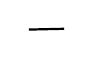
\begin{tikzpicture}[baseline=0pt]\draw[line width=.8pt] (0,0)--(.45,.01);\end{tikzpicture}}

\uline{Proposition 2} Soit $Y'$ une surface orientée de t.f. (\inserted{surf.} cpte $-$ nb fini de pts) \uline{anabélienne}, i.e. telle que pour tte comp. connexe $Y'_i$ de $Y'$, on ait $\chi_!(Y'_i)<0$ (i.e. on ait $2g_i+\nu_i\geq 3$, où $g_i$ est le genre de $Y'_i$ et $\nu_i$ le nb des trous\ldots). Alors tout autom. \inserted{$\gamma$} d'ordre fini de $Y'_i$ qui est isotope à l'identité est l'identité.

Comme $\gamma$ invarie les composantes connexes, OPS $Y'$ connexe. En fait, il suffit que $\gamma$ opère trivialement sur la homologie \inserted{$H_1$} (\inserted{p.ex.} à coefficients dans $\mathbb{Z}$, ou dans \inserted{un} $\mathbb{Z}/n\mathbb{Z}$ avec $n\geq3$) pour
\margin{4}
\scanpage{6}
factoriser \uline{canoniquement} en
\diagram{
\begin{tikzcd}[ampersand replacement=\&]
(10)\quad X \arrow[r,"{\substack{f_0\\[-2pt]\sim}}"] \& Y' \arrow[r,"p"] \& Y
\end{tikzcd}
}
où $Y'$ est un rev. étale fini de $Y$, défini à isom. unique près, et où $X\xrightarrow{\sim}Y'$ est un isom dans la cat. isotopique -- i.e. une classe d'isotopie d'homéomorphismes ? Bien sûr, si on n'a pas une d'exigence de canonicité, la factorisabilité (10) de $f$ est triviale -- il suffit de prendre un représentant quelconque de $f$. \deleted{Plus} Pour préciser la \deleted{question} condition d'unicité, on est amené à se poser la question si pour tt $Y$-autom. \deleted{$\unsure{g}$} \inserted{$\gamma$ de $Y'$} \deleted{la \unsure{condition|classe}} (\uline{pas} à isot. près !) \deleted{tel que l'on ait} on a l'implicat°
\[
(11)\qquad (\gamma f_0\sim\deleted{\unsure{\gamma}}f_0)\Longrightarrow\gamma=\operatorname{id}_{Y'}\quad ?
\]
Dans cette question, on peut bien sûr supposer $f_0=\operatorname{id}$, donc la question est si un autom d'ordre fini \inserted{$\gamma$} d'\deleted{une} \inserted{la} surface orientée $Y'$ de type fini, qui est isotope à l'identité, est l'identité.

La condition supplémentaire, que $\gamma$ est un $Y$-autom., où $Y'\mathbin{-}Y$ est fini étale, signifie aussi que $\gamma$ opère via une opération \uline{libre} de $\mathbb{Z}/n\mathbb{Z}$ (où $n$ est l'ordre de $\gamma$) -- mais en admettant que si $\gamma$ \inserted{(autom. d'ordre fini)} n'est pas l'identité, ses pts fixes sont isolés,
\margin{5}
\scanpage{7}
\mspage{3}
que $\gamma$ soit l'identité. Pour le voir, on peut supposer que $\gamma$ laisse invariante une structure \deleted{de} de courbe algébrique (de type $(g,\nu)$ anabélien) sur $X$. Il suffit \deleted{de} que l'on ait $2g-\nu\geq2$, i.e. que $X$ se plonge dans \unsure{une|sa} jacobienne généralisée, ext. d'une VA par un tore, pour pouvoir conclure de l'hypothèse homologique que $\gamma$ \deleted{est} induit une \uline{translation} sur cette jacobienne, par un élément d'ordre fini de la jacobienne homogène. Il faut donc voir que $X$ plongé dans sa jacobienne n'est stable par aucune \deleted{\unsure{autom.}} translation non nulle, dans le cas anabélien -- c'est là un fait bien connu\ldots\ [Sûrement, il ne doit pas être difficile de trouver une démonstration purement topologique de la proposition précédente\ldots]

Notons maintenant que si $Y$ est une surface \inserted{top} anabélienne, tout revêtement étale fini l'est également. On trouve donc le

\deleted{\uline{Proposition}} \inserted{Corollaire} 3\quad Soient $X,Y$ \deleted{deux} comme plus haut, \inserted{$Y$-anabélienne}.
Alors toute classe d'isotopie de morphismes finis étales de $X$ dans $Y$ est un \uline{torseur} à droite sous le groupe $\mathcal{A}_X^0$ des autom de $X$ isotopes à l'identité.

Compte tenu de la proposition 1, il reste
\margin{6}
\scanpage{8}
à prouver que si $f:X\mathbin{-}Y$ fait de $X$ un rev. fini étale de $Y$ et si $u\in\mathcal{A}_X^0$ est tel que $f=f\circ u$ i.e. $u$ est un $Y$-morphisme, alors $u=\operatorname{id}$. Mais c'est ce qu'affirme la prop. 2.

\uline{Corollaire 2} Les composantes connexes de l'espace des morphismes finis étales $X\longrightarrow Y$ sont contractiles.

\uline{Corollaire 3} \deleted{L'ensemble $\operatorname{Hom}_{\mathrm{isot}}(X,Y)$ est un torseur \inserted{\deleted{à droite}} sous le} \inserted{L'opération à droite du} groupe de Teichmüller (non orienté) $\mathcal{T}_X=\mathcal{A}_X/\mathcal{A}_X^0$ sur l'ens $\operatorname{Hom}_{\mathrm{isot}}(X,Y)$ des ``morphismes isotopiques'' de $X$ dans $Y$ \deleted{est libre,} a des stabilisateurs qui sont des sous-groupes finis de $\mathcal{T}_X$.
\margin{\uline{NB} Tout sous-groupe fini de $\mathcal{T}_X$ peut s'obtenir de cette façon comme stabilisateur !! (Th. profond et récent\ldots)}

De façon précise, le stabilisateur de $f\in\operatorname{Hom}_{\mathrm{isot}}(X,Y)$ s'identifie au \deleted{un} \inserted{groupe} \deleted{gr.} des $Y$-autom. du rev. fini étale $Y'_f$ défini par $f$. L'ensemble des orbites de $\mathcal{T}_X$ opérant sur $\operatorname{Hom}_{\mathrm{isot}}(X,Y)$ est en corr. biunivoque avec l'ens \inserted{$\deleted{\operatorname{Rev}_X(Y)}\ \mathcal{R}_X(Y)$} des classes d'isom. de revêtements finis étales de $Y$, homéomorphes à $X$.
\margin{\uline{NB} cet ens d'orbites est \uuline{fini}}
\margin{\figure{\begin{tikzpicture}[baseline=0pt]\draw (0,0)--(0,2.1);\end{tikzpicture}}}
[L'ens des orbites sous $\mathcal{T}_X^+$ est en corr. biunivoque avec l'ens. $\mathcal{R}_X(Y)\times\{\pm1\}$, le signe $+$ resp. $-$ correspondant aux classes de morphismes finis étales $X\longrightarrow Y$
\margin{7}
\scanpage{9}
\mspage{4}
qui conservent resp. renversent l'orientation, i.e.
\[
\operatorname{Hom}_{\mathrm{isot}}^+(X,Y)\quad\text{et}\quad\operatorname{Hom}_{\mathrm{isot}}^-(X,Y).
\]
\deleted{Supposons maintenant}

\uline{Scholie} Par la composition évidente des $\operatorname{Hom}_{\mathrm{isot}}^+(X,Y)$, les surfaces topologiques orientées anabéliennes (i.e. de t.f. et anabéliennes) \deleted{anabéliennes} forment une catégorie, la ``catégorie isotopique orientée'' des surfaces orientées anabéliennes. \deleted{La catégorie $X$ et $Y$ deux surfaces anabéliennes, \unsure{le de}} \inserted{Il y a équiv. entre la catégorie-groupoïde} des triplets $(X,Y,f)$ de deux surfaces top. anabéliennes $X,Y$ et d'un $f\in\operatorname{Hom}_{\mathrm{isot}}^+(X,Y)$, et celle des quadruplets $(X,Y,Y',f_0)$, où $X$ et $Y$ sont itou, $Y'$ un rev. étale fini de $Y$, et $f_0$ est une classe d'isotopie d'un isom. orienté de $X$ et $Y'$, i.e. $f_0\in\operatorname{Isom}_{\mathrm{isot}}^+(X,Y')$.

Posons maintenant
\margin{Pour la suite, on laisse tomber le $+$ dans les notations -- tous les morphismes étales envisagés conservent l'orientation.}
\[
(12)\quad
\widehat{\operatorname{Hom}}^{+}_{\mathrm{isotop}}(X,Y)
=\overbrace{\operatorname{Hom}^{+}_{\mathrm{isot}}(X,Y)\mathop{\wedge}_{\mathcal{T}_X}
\underbrace{\widehat{\mathcal{T}}_X}_{\text{compactifié profini}}}^{\substack{\text{muni de la topologie}\\\text{somme d'espaces compacts}}}
\]
\margin{[Somme \inserted{\uline{finie}} d'ailleurs -- donc $\widehat{\operatorname{Hom}}$ est cpct\ldots]}
On définit une composition
\[
(13)\quad\left\{
\begin{aligned}
\widehat{\operatorname{Hom}}_{\mathrm{isot}}(X,\unsure{Y|Z})\times
\widehat{\operatorname{Hom}}_{\mathrm{isot}}(X,Z)
&\mathbin{-}\widehat{\operatorname{Hom}}_{\mathrm{isot}}(X,Z)\\
\text{contin}\qquad (u,v)&\longmapsto v\circ u
\end{aligned}\right.
\]
\margin{8}
\scanpage{10}
satisfaisant à la propriété d'associativité évidente, \unsure{par|pour} prolongement par continuité à partir de l'accouplement au niveau des $\operatorname{Hom}$ sans $\hat{\ }$. \deleted{La construction marche dans tous}

\margin{Mérite d'être fait avec plus de soin !}
\uline{Digression axiomatique}\quad Une catégorie $\mathcal{C}$ est dite \deleted{``à $\operatorname{Hom}$ profinis'' si les $\operatorname{Hom}$} \deleted{``à $\operatorname{Hom}$''} ``à \deleted{autom} \inserted{groupes d'autom.} profinis'' si pour tt $X\in C$, $\operatorname{Aut}X$ est muni d'une structure de groupe profini, de telle façon que pour tout $u:X\longrightarrow Y$ de $C$, les stabilisateurs de $u\in\operatorname{Hom}_C(X,Y)$ dans $\operatorname{Aut}_C(X)\times\operatorname{Aut}_C(Y)$ \deleted{à} \inserted{opérant par $u\longmapsto guf^{-1}$,} \deleted{droite) et $\operatorname{Aut}_C(Y)$ (opère à g.) sont des} sous-groupes fermés. \deleted{On} On munit alors chaque orbite de $\operatorname{Hom}(X,Y)$ sous $\operatorname{Aut}(X)\times\operatorname{Aut}(Y)$ de la topologie profinie quotient, et $\operatorname{Hom}(X,Y)$ de la topologie \inserted{disjointe} somme des orbites, de sorte que $\operatorname{Hom}(X,Y)$ devient un espace loc. compact.

Je \deleted{\unsure{dis}} \inserted{veux} que l'accouplement des morphismes
\[
(14)\quad\left\{
\begin{aligned}
\operatorname{Hom}(X,Y)\times\operatorname{Hom}(Y,Z)&\mathbin{-}\operatorname{Hom}(X,Z)\\
(u,v)&\longmapsto vu
\end{aligned}\right.
\]
est alors \deleted{continue} une \deleted{morphi.} application continue. Il suffit de le voir sur des produits d'orbites, donc de voir que \inserted{pour $u,v$ fixés,} l'application
\[
\begin{gathered}
(g,f,g',f')\longmapsto(g'vf'^{-1})\circ(guf^{-1})\\
\operatorname{Aut}(Z)\times\operatorname{Aut}(X)\times\operatorname{Aut}(Z)\times\operatorname{Aut}(Y)\longrightarrow\operatorname{Hom}(X,Z)
\end{gathered}
\]
\margin{9}
\scanpage{11}
\margin{10}
\mspage{5}
est continue. Il revient au $=$ que l'application
\[
(15)\qquad\begin{aligned}
\operatorname{Aut}(Y)&\longrightarrow\operatorname{Hom}(X,Z)\\
\varphi&\longmapsto v\varphi u
\end{aligned}
\]
soit continue.

Considérons \deleted{alors et} le stabilisateur \deleted{de}
$G_u$ de $u\in\operatorname{Hom}(X,Y)$ dans $\operatorname{Aut}(X)\times\operatorname{Aut}(Y)$
\[
\begin{aligned}
G_u&\subset\operatorname{Aut}(X)\times\operatorname{Aut}(Y)\\
\rotatebox{90}{$=$}\quad&\\[-1ex]
\{\psi,\varphi\mid\varphi u\psi^{-1}=u\quad\text{i.e.}\quad\varphi u=u\psi\}&
\end{aligned}
\]
c'est un sous-groupe fermé de $\operatorname{Aut}(X)\times\operatorname{Aut}(Y)$,
et l'application composée
\diagram{\begin{tikzcd}[ampersand replacement=\&]
G_u\arrow[r,"\mathrm{pr}_2"]\&\operatorname{Aut}(Y)\arrow[r]\&\operatorname{Hom}(X,Z)
\end{tikzcd}}
n'est autre que $(\psi,\varphi)\longmapsto v\varphi u=\uline{vu}\psi$, qui est
donc continue, par construction de la top. de
$\operatorname{Hom}(X,Z)$. Donc l'application $\operatorname{Aut}(Y)\longrightarrow\operatorname{Hom}(X,Z)$
est continue en tous cas sur l'image \inserted{$H_u\subset\operatorname{Aut}(Y)$} de $G_u$
par $\mathrm{pr}_2$, \inserted{(car la top. de cette image est quotient de celle de $G_u$)} donc aussi sur tte réunion
finie de translatés à gauche \inserted{$\alpha_iH_u$ $(\alpha_i\in\operatorname{Aut}(Y))$} de cette image,
puisque l'on aura \deleted{\unsure{on}}
\[
v(\alpha_i\varphi)u=v\alpha_i u\psi.
\]
\margin{\uline{NB} $H_u$ est un sous-groupe \uuline{fermé} de $\operatorname{Aut}(Y)$, donc il est ouvert s'il est d'indice fini\ldots}
Donc la continuité de (14), donc de (15), est
acquise, si on fait l'hypothèse :
\[
(16)\quad(*)\quad\left\{
\begin{minipage}{0.83\linewidth}
Pour toute flèche $u:X\mathbin{-}Y$ dans $C$, l'image
$H_u$ dans $\operatorname{Aut}_C(Y)$ du groupe $G_u$ des automs de cette
\inserted{flèche} est un sous-groupe d'\uline{indice fini de}
$\operatorname{Aut}(Y)$.
\end{minipage}\right.
\]
\margin{\uline{NB} L'hypothèse (16) implique que \inserted{dans} $\operatorname{Hom}(X,Y)$, les \deleted{\unsure{classes}} orbites \uline{sous} $\operatorname{Aut}(X)$ sont déjà ouvertes, tte orbite sous $\operatorname{Aut}_{0}(X)\times\operatorname{Aut}_{\unsure{1}}(Y)$ étant réunion finie de telles orbites\ldots}
\scanpage{12}
Soit maintenant $C_0$ une catégorie (sans
données topologiques préalables sur $C_0$),
telle que $C_0$ satisfasse la condition
qui correspond à $(*)$ (condition qui ne
fait pas appel à des données topologiques).
Je dis qu'on peut alors trouver une
solution au Pb d'envoyer $C_0$, par un foncteur,
dans une catégorie \inserted{$C$} ``essentiellement profinie''
[i.e. où les $\operatorname{Hom}_C(X,Y)$ sont des espaces loc. compacts
séparés, \inserted{où on a la continuité pour la composition}, les $\operatorname{Aut}_C(X)$ sont --- pour la topologie
induite par $\operatorname{Hom}(X,X)\times\operatorname{Hom}(X,X)$ --- des
\inserted{$\operatorname{Aut}(X)\simeq\{(u,v)\mid uv=\mathrm{id},\ vu=\mathrm{id}\}$}
groupes profinis, et les orbites des $\operatorname{Aut}(X)\times\operatorname{Aut}(Y)$
dans $\operatorname{Hom}_C(X,Y)$ sont ouvertes\ldots], en prenant
\margin{devrait \unsure{suffire}\quad\figure{\begin{tikzpicture}[baseline=0pt]\draw (0.6,0)--(0.6,2.1);\draw[->] (0,1.2)--(0.55,1.2);\end{tikzpicture}}}
comme ``enveloppe profinie'' $\widehat C_0$ \deleted{définie} ayant les
$=$s \deleted{$C_0$} objets que $C_0$, et en prenant
\diagram{\begin{tikzcd}[ampersand replacement=\&,column sep=small,row sep=large]
(17)\quad\operatorname{Hom}_{\widehat C_0}(X,Y)=\&\operatorname{Hom}_{C_0}(X,Y)\mathbin{\wedge}_{\operatorname{Aut}(X)\times\operatorname{Aut}(Y)^0}\widehat{\operatorname{Aut}}(X)\times\widehat{\operatorname{Aut}}(Y)\\
\&\deleted{\unsure{\simeq}}\operatorname{Hom}_{C_0}(X,Y)\mathbin{\wedge}_{\operatorname{Aut}(X)}\widehat{\operatorname{Aut}}(X)\arrow[u,"\sim"]
\end{tikzcd}}
\figure{\begin{tikzpicture}[baseline=0pt]\draw (1.4,0.7)..controls (1.3,0.35) and (0.3,0.1)..(0,0);\fill (1.18,0.67) circle (0.015);\end{tikzpicture}}
\margin{avec la top. d'espace somme d'espaces compacts\ldots}
la composition des morphismes de $\widehat C_0$ se
définissant ad-hoc (de façon unique, d'ailleurs,
en exigeant la continuité de la composition, et
qu'elle prolonge celle donnée sur $C_0$).
Par construction, tout $\widehat C_0$-morphisme
\margin{11}
\scanpage{13}
\mspage{6}
Revenons au cas de la catégorie isotopique
des surfaces orientées \deleted{de t.f.} \inserted{anabéliennes}, il lui est donc
associée une catégorie ``compactifiée profinie'',
avec des $\operatorname{Hom}^{\wedge}$ \inserted{donnés par} (12) --- ce sont
\deleted{(à $\Pi_0$ compts dénombrables)}
des espaces sommes top. d'espaces compacts
totalement discontinus --- en fait, ce sont
des espaces loc. compacts dénombrables à l'infini,
totalement disconnexes, métrisables --- toutes
les qualités ! (Et pas de pts isolés, par
surcroît\ldots)

Limitons-nous maintenant au cas des
surfaces $X$ qui sont munies d'une structure
de courbe alg. complexe, compatible avec sa
topologie. Alors les morphismes entre tels
$X$, dans un $\operatorname{Hom}^{\wedge}_{\mathrm{isot}}$, et leur composition,
définis ici en utilisant de façon essentielle
la topologie du corps des complexes $C$
(permettant d'associer aux schémas en courbes
lisses quasi-projectives sur $C$ des surfaces
topologiques orientées de t.f.), peuvent se
décrire de façon purement algébro-géomé-
trique, indépendamment de cette topologie
de $\mathbb C$ (cas anabélien, tjrs). Pour le
\margin{12}
\scanpage{14}
\[
(18)\qquad\widehat f:\overset{\deleted{\wedge}}{X}\mathbin{-}Y
\]
se factorise en
\diagram{\begin{tikzcd}[ampersand replacement=\&]
(19)\quad X\arrow[r,"\widehat f_0","\sim"']\&Y'\arrow[r,"u"]\&Y
\end{tikzcd}}
où $u$ est un $C_0$-morphisme, et $\widehat f_0$ un $\widehat C_0$-\uline{isomorphisme}
(\uline{NB} $Y'$ est un objet $C_0$-isom. à $X$), et où $u$ est
un morphisme de $C_0$. Dans le cas où on
suppose que pour toute flèche $u:Y'\mathbin{-}Y$ dans $C$,
l'hom. composé
\diagram{\begin{tikzcd}[ampersand replacement=\&]
\operatorname{Aut}_Y(Y')\arrow[r]\&\operatorname{Aut}(Y')\arrow[r,no head]\&\operatorname{Aut}(Y')^{\wedge}
\end{tikzcd}}
\uline{injectif}, on voit que $Y'$ est déterminé
en termes de $\widehat f$ à $Y$-isom. unique près. \deleted{De} La
\inserted{recette} \deleted{plus, pour} pour composer deux morphismes définis
ainsi, $\widehat f=u\widehat f_0$ et $\widehat g=v\widehat g_0$
\margin{\uline{NB} Le foncteur can $C_0\longrightarrow\widehat C_0$ est conservatif (i.e. $\widehat f_0$ est $C_0$-iso $\Longleftrightarrow$ c'est un $\widehat C_0$-iso) \deleted{De \unsure{plus}} \inserted{plus,} Tout $\widehat C_0$-isom. est limite de $C_0$-isom.\ldots\ de façon précise,
$\operatorname{Isom}_{\widehat C_0}(X,Y)\simeq\operatorname{Isom}_{C_0}(X,Y)\mathbin{\wedge}_{\operatorname{Aut}_{C_0}(X)}\widehat{\operatorname{Aut}}_{C_0}(X)$
et $\operatorname{Aut}_{\widehat C_0}(X)\simeq\widehat{\operatorname{Aut}}_{C_0}(X)$.}
\diagram{\begin{tikzcd}[ampersand replacement=\&]
(20)\quad Y\arrow[r,no head,"\deleted{\unsure{g}}\widehat g_0","\sim"']\&Z'\arrow[r,no head,"v"]\&Z,
\end{tikzcd}}
et les mettre sous la $=$ forme standard,
est le suivant : on approche $\widehat g_0:Y\overset{\sim}{\longrightarrow}Z'$
(qui est un $\widehat C_0$-iso) par
un \deleted{vrai} \inserted{$C_0$-iso} morphisme \deleted{$\unsure{u}$} $w$
de telle façon que l'on ait
\[
\widehat g_0=w\widehat\varphi\qquad\text{avec}\quad\widehat\varphi\in\widehat H_u\subset\widehat{\operatorname{Aut}}_{C_0}(Y)
\]
\diagram{\begin{tikzcd}[ampersand replacement=\&,column sep=small]
\&\&Y'\arrow[r,"u"]\&Y\arrow[dr,"w"]\&\&\\
(21)\quad X\arrow[r,no head,"\widehat f_0","\sim"']\&Y'\arrow[r,"u"]\arrow[ur,"\widehat\psi?" ]\&Y\arrow[rr,"\widehat g_0","\sim"']\arrow[ur,"\widehat\varphi?"]\&\&Z'\arrow[r,"v"]\&Z
\end{tikzcd}}
\margin{\uline{NB} Il faut savoir interpréter en termes de $C_0$ déjà \figure{\begin{tikzpicture}[baseline=0pt]\draw (0,0)--(.35,0);\draw (0,.08)--(.35,.08);\end{tikzpicture}} la relation $\widehat\varphi u=u\widehat\psi$ comme signifiant $(\widehat\psi,\widehat\varphi)\in\widehat G_u$, où $G_u\subset\operatorname{Aut}(X)\times\operatorname{Aut}(Y)$ est le stabilisateur de $u$\ldots}
(ce qui est possible, puisque $\widehat H_u$ est ouvert dans $\widehat{\operatorname{Aut}}_{C_0}(Y)$),
et on choisit $\widehat\psi\in\widehat{\operatorname{Aut}}(Y')$ tel qu'on ait $\widehat\varphi u=u\widehat\psi$
donc on aura
\[
(22)\qquad\widehat g\widehat f=(v\widehat g_0)(u\widehat f_0)
=(v\deleted{\unsure{g}}w\widehat\varphi)(u\widehat f_0)
=\underbrace{(vwu)}_{\in\mathrm{Fl}\,C_0}\underset{\in\mathrm{Flisom.}(\widehat C_0)}{\underline{(\widehat\psi\widehat f_0)}}
\]
\margin{13}
\scanpage{16}
pour des hom de corps, par des foncteurs
de ``changement de base'' pour $k\mathbin{-}k'$
qui sont d'ailleurs \deleted{pl. fidèles} \inserted{des équiv. de cat.} [mais
pas \deleted{essentiellement} surjectifs]. (Cela provient
du fait que le groupoïde fondamental
de' \deleted{\unsure{une}} \inserted{la} multiplicité modulaire pertinente,
ou d'une courbe alg., sur un corps alg.
clos $k$, ne change pas à équiv. près
par l'extension $k\mathbin{-}k'$ du corps de base,
avec $k'$ alg. clos) \deleted{par contre il y a \unsure{encore},
si $k'\ne k$, des courbes alg.}
\margin{Mais cela ne signifie bien sûr \inserted{pas} que $\forall$ courbe alg. sur $k'$ soit isom. sur $k'$ à une courbe provenant de $k$ !}

En particulier, le groupe des automorphis-
mes de $k$ opère sur la catégorie précédente,
que j'ai envie d'appeler la \uline{catégorie de
Teichmüller-Galois} associée à $k$. Les
\deleted{objets} \inserted{classes d'iso.} d'objets connexes de cette
catégorie sont en corr. $1$-$1$ avec les types
$(g,\nu)$ des courbes anabéliennes; les groupes
d'automorphismes d'un objet sont essentielle-
ment (en car. $0$ du moins) des compactifiés
profinis des groupes de Teichmüller st.-ext.
\margin{15}
\scanpage{17}
\mspage{8}
Le fait d'avoir élargi le \uline{groupoïde} de
Teichmüller-Poincaré en la catégorie (qui n'est
plus un groupoïde !) de Teichmüller-
Galois précédente, est une façon \deleted{commode} \inserted{naturelle}
pour relier entre eux des courbes alg. relatifs
à des types numériques $(g,\nu)$ différents.
Une part essentielle de mon ``programme
à l'horizon'' est de déterminer de façon
plus ou moins complète cette catégorie
de Galois-Teichmüller, \inserted{par voie ``algébrique'' (ni transcendante ni de géométrie algébrique !)} \uline{avec} \uline{les opérations}
de $\operatorname{Aut}k$ \uline{dessus}, tout au moins dans
le cas où $k=\overline{\mathbb Q}$, et aussi (dans une
certaine mesure) lorsqu'on prend \deleted{des}
$k=\overline K$, $K$ corps de type fini sur $\unsure{Q|\mathbb Q}$, et
qu'on se limite aux \deleted{$K$}-automs \inserted{de $\overline K$} qui
sont des $K$-automs.\ldots\ (?).
\margin{``algébrique'' devant signifier ici : par des méthodes de topologie surfaces, de \uline{combinatoire} (cartes) et des méthodes de théorie des groupes profinis\ldots}
\margin{16}
\scanpage{18}
Dans tout ceci, il reste cependant un
type important de \deleted{\unsure{hom.}} morphismes, entre
surfaces \inserted{top.} comp. clos ou entre schémas en
courbes, qui n'a pas été pris en ligne
de compte --- savoir les morphismes
d'inclusion ouverte
\diagram{\begin{tikzcd}[ampersand replacement=\&]
(23)\quad X=Y\setminus T\arrow[r,hook,no head]\&Y
\end{tikzcd}}
correspondants à une opération de \uline{bouchage
de trous}. Mais on est confronté, pour élargir la
catégorie en conséquence, par l'impératif de
pouvoir composer les morphismes étales finis,
et d'inclusion ouverte (type ``bouchage de trous'')
à envisager des morphismes $X\longrightarrow Y$ qui
s'insèrent dans un diagramme commutatif
\diagram{\begin{tikzcd}[ampersand replacement=\&]
X\arrow[r,hook,no head]\arrow[d]\&\widehat X\arrow[d]\\
(24)\quad Y\arrow[r,hook,no head]\&\widehat Y
\end{tikzcd}}
avec $\widehat X\longrightarrow\widehat Y$ fini ramifié, $X\mathbin{-}Y$ lui-$=$ étale.
Posant $S=\widehat X\setminus X$, $T=\widehat Y-T$, de sorte que
\[
(25)\qquad S\supset\widehat X|T
\]
les ennuis techniques proviennent du fait que
l'on est obligé d'admettre que $\widehat X/\widehat Y$ puisse avoir des
pts de ramification effective non seulement en
des pts de $\widehat X|T$, mais aussi en des pts de $C$ qui
ne sont \uline{pas} dans $\widehat X|T$.
\margin{17}
\scanpage{19}
\mspage{9}
La notion d'isotopie raisonnable pour des
tels morphismes (dans le contexte topologique),
se trouve être équivalente à la congruence
sous le groupe $\operatorname{Aut}^0(X)\times\operatorname{Aut}^0(Y)$
(où $\operatorname{Aut}^{\deleted{\unsure{0}}}(X)$ est interprété comme $\operatorname{Aut}(\widehat X,S)$,
et $\operatorname{Aut}(Y)$ comme $\operatorname{Aut}(\widehat Y,T)$). L'ennui,
c'est qu'il n'y a plus de factorisation
\uline{canonique} d'une classe d'isotopie des
morphismes \inserted{$X\longrightarrow Y$} (dont les éléments \inserted{variables} $f$
transforment $S_1=S\setminus S_0$ où $S_0=\widehat X|T$) en
des parties variables de $Y=\widehat Y\setminus T$) en
une isomorphisme \deleted{suivi} isotopique \deleted{suivi} \inserted{ou plutôt}
\inserted{une classe d'isotopie d'inclusions type ``bouchage de trous'',}
\inserted{suivi} d'un morphisme $Y'\longrightarrow Y$, où $Y'$ est un
morphisme fini (possédant maintenant aussi
\inserted{en plus} des pts de ramification, au dessus des
points de $Y$ qui \uline{ne sont pas} déterminés
par la classe seule). Pour cette raison,
je ne vois plus comment interpréter une
telle classe, ou son image dans un
\deleted{``\unsure{complétifié|complété} profini''} ``complété profini'' convenable,
en termes de géom. alg. ``abstraite'' sur $\mathbb C$,
\margin{18}
\scanpage{20}
lorsque $X$ et $Y$ sont des courbes \uline{algébriques}
anabéliennes sur $\mathbb C$.

Pourtant, il \deleted{doit être} \inserted{est} possible tout au
moins, sur un corps alg. \inserted{clos $k$} quelconque,
de définir un \uline{foncteur} qui va du
\uline{groupoïde} de Teichmüller des
courbes de type $(g,\nu)$, \inserted{(disons)} avec un
paquet \deleted{de} $I$ de cardinal $\nu'\leq\nu$ de
pts épinglés par $I$, vers le \uline{groupoïde}
de Teichmüller de type $(g,\nu-\nu')$,
par ``bouchage des trous en $I$'', \deleted{\unsure{cela} dit, si}
avec \deleted{\unsure{une|les}} \unsure{propriétés|propriété} de transitivi-
té évidents, pour des bouchages de
trous successifs. Mais je vois malaisé-
ment comment l'inclure dans une
notion correspondante de ``morphismes d'
inclusion'', qui pourrait se composer
avec les morphismes dont on dispose
déjà dans la \uline{catégorie} (pas groupoïde !)
de Galois-Teichmüller. À moins d'y
\margin{19}
\scanpage{21}
\mspage{10}
aller comme une brute et de définir
une catégorie plus grosse que la cat.
de Galois-Teichmüller (i.e. à ens
de flèches plus gros) par \uline{générateurs}
et relations convenables. Mais alors il
devient problématique, quand le corps de
base est le corps $\mathbb C$ des complexes, d'
interpréter cette catégorie de Galois-Teich-
müller comme une ``complétée profinie''
de la catégorie isotopique envisagée plus
haut.
\margin{20}
\scanpage{22}
\margin{40 pags}
Opérations de $\mathbf{\Gamma}_{\overline{\mathbb Q}/\mathbb Q}$
sur $\deleted{\unsure{C|\Pi}}\mathbf{\Pi}_1\mathbf U_{03}$
\margin{21}
\scanpage{24}
\mspage{(5)}
\figure{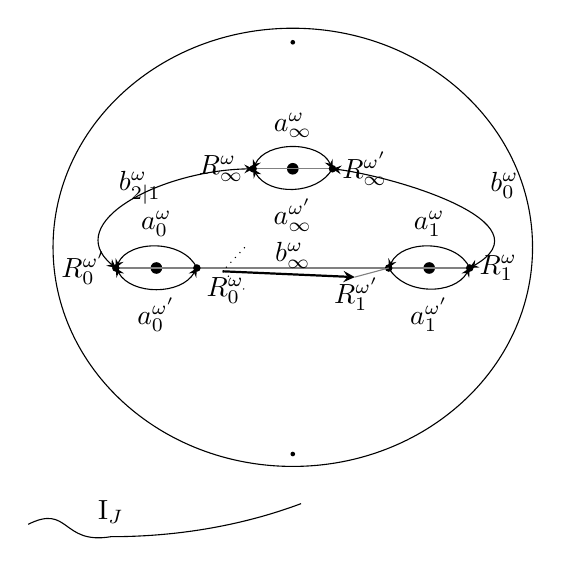
\begin{tikzpicture}[scale=1.05,>=stealth]
\draw[thin] (0,0) ellipse (2.9 and 2.65);
\fill (0,2.48) circle (.8pt);\fill (0,-2.5) circle (.8pt);
\fill (0,0.95) circle (2pt);\fill (-1.65,-0.25) circle (2pt);\fill (1.65,-0.25) circle (2pt);
\coordinate (ti) at (-.48,.95);\coordinate (tp) at (.48,.95);
\coordinate (li) at (-1.16,-.25);\coordinate (lp) at (-2.14,-.25);
\coordinate (ri) at (2.14,-.25);\coordinate (rp) at (1.16,-.25);
\draw[thin,gray] (ti)--(tp);\draw[thin,gray] (lp)--(ri);
\foreach \p in {ti,tp,li,lp,ri,rp}{\fill (\p) circle (1.3pt);}
\draw[<->] (ti) to[bend left=65] node[above] {$a_\infty^\omega$} (tp);
\draw[->] (tp) to[bend left=60] node[below] {$a_\infty^{\omega'}$} (ti);
\draw[->] (li) to[bend right=65] node[above] {$a_0^\omega$} (lp);
\draw[<->] (lp) to[bend right=60] node[below] {$a_0^{\omega'}$} (li);
\draw[->] (ri) to[bend right=65] node[above] {$a_1^\omega$} (rp);
\draw[->] (rp) to[bend right=60] node[below] {$a_1^{\omega'}$} (ri);
\draw[<->] (ti) .. controls (-1.6,.93) and (-2.8,.30) .. (lp);
\node at (-1.85,.72) {$b_{\unsure{2|1}}^\omega$};
\draw[<->] (ri) .. controls (3.1,.3) and (1.25,.85) .. (tp);
\node at (2.56,.75) {$b_0^\omega$};
\draw[dotted] (-.58,0)--(-.85,-.29)--(-.55,-.54);\draw[->,thick] (-.85,-.29)--(.75,-.36);
\draw[thin,gray] (.75,-.36)--(rp);\node at (0,-.10) {$b_\infty^\omega$};
\node[left] at (ti) {$R_\infty^\omega$};\node[right] at (tp) {$R_\infty^{\omega'}$};
\node[left] at (lp) {$R_0^{\omega'}$};\node[below right] at (li) {$R_0^\omega$};
\node[below left] at (rp) {$R_1^{\omega'}$};\node[right] at (ri) {$R_1^\omega$};
\node at (-2.2,-3.2) {$\mathrm I_J$};
\draw (-3.2,-3.35) .. controls (-2.7,-3.1) and (-2.8,-3.6) .. (-2.2,-3.5) .. controls (-1.1,-3.5) and (-.3,-3.25) .. (.1,-3.1);
\end{tikzpicture}}
$\mathcal G_J$ permute transitivement les six flèches $a_i^\omega$ et les six flèches $b_i^\omega$ : \deleted{$R$}
\[
(1)\quad\left\{\begin{aligned}
a_i^\omega &: R_i^\omega\mathbin{-}R_i^{\omega'}\\
b_i^\omega &: R_{\omega i}^\omega\longrightarrow R_{\omega'i}^{\omega'}
\end{aligned}\right.
\]
\[
(2)\quad\left\{\begin{aligned}
\mathrm a)\quad &b_i^\omega b_i^{\omega'}=1&&\text{(trois relations effectives)}\\
\mathrm b)\quad &a_i^\omega b_{\omega'i}^{\omega}a_i^{\omega'}b_{\omega i}^{\omega}
a_{\omega'i}^{\omega'}b_i^\omega=1&&\text{(deux relations effectives, une pour chaque }\omega\in\uline{\omega}\text{)}
\end{aligned}\right.
\]
\margin{\uuline{NB}\quad $\tau(R_i^\omega)=R_i^\omega$\quad $\tau(a_i^\omega)=(a_i^{\omega'})^{-1}$\quad $\tau(b_i^\omega)=b_i^\omega$.}
\[
(3)\quad a_i^{\omega'}a_i^\omega=\lambda_i^\omega=\varphi_i^\omega(l_0)
\]
\diagram{\begin{tikzcd}[ampersand replacement=\&,column sep=small,row sep=small]
(4)\quad\varphi_i^\omega:\quad\Pi_{03}\arrow[dr,bend right=15]\&{}=\Pi_1(U_{0,3};R_0^+)=\{l_0,l_1,l_\infty\mid l_\infty l_1l_0=1\}\subset\widetilde\Pi_{0,3}=\Pi_1(U_{0,3},\mathcal G_J;R_0^+\unsure{)}\\
\&\Pi_1(\Sigma^*,R_i^\omega)
\end{tikzcd}}
\[
\begin{aligned}
l_0&\longmapsto a_i^{\omega'}a_i^\omega\\
l_1&\longmapsto (\unsure{b_{\omega i}^\omega|b_\infty^\omega})^{-1}\underbrace{a_{\omega i}^{\omega}a_{\omega i}^{\omega'}b_i^\omega}
\end{aligned}
\]
Les $\varphi_i^\omega$ sont permutés entre eux de façon simplement transitive
\[
(5)\quad\tau\varphi_i^\omega(g)=\varphi_i^\omega(\tau_\infty(g))
\qquad\text{où}\quad\tau_\infty\in\widetilde\Pi_{0,3}
\qquad\left\{\begin{aligned}
\tau_\infty(l_0)&=l_0^{-1}\\
\tau_\infty(l_1)&=l_1^{-1}\\
\tau_\infty(l_\infty)&=l_0l_1=\operatorname{int}(l_0)l_\infty^{-1}
\end{aligned}\right.
\]
\[
(6)\quad\left\{\begin{aligned}
a_i^\omega(\varphi_i^\omega(g))&=\varphi_i^{\omega'}(\varepsilon_0(g))\\
b_i^\omega(\varphi_{\omega i}^\omega(g))&=\varphi_{\omega'i}^{\omega'}(\sigma_\infty(g))
\end{aligned}\right.
\qquad\varepsilon_0^2=l_0
\]
\margin{\figure{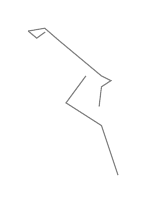
\begin{tikzpicture}[scale=.6]
\draw[gray,thin] (0,2.6)--(.35,2.66)--(.65,2.4)--(1.55,1.65)--(1.75,1.55)--(1.55,1.42)--(1.5,1.0);
\draw[gray,thin] (1.22,1.65)--(.8,1.08)--(1.55,.6)--(1.9,-.45);
\draw[gray,thin] (0,2.6)--(.18,2.45)--(.36,2.58);
\end{tikzpicture}}}
\[
\begin{aligned}
\sigma_\infty(l_0)'&=l_1\\
\sigma_\infty(l_1)&=l_0\\
\sigma_\infty(l_\infty)&=(l_0l_1)^{-1}=l_1^{-1}l_0^{-1}=\operatorname{int}(l_0)l_\infty
\end{aligned}
\]
\deleted{$\unsure{\widetilde b_{\omega'i}^\omega|\widetilde b_i^\omega}$}

On introduit
\[
(7)\quad\widetilde b_i^\omega=a_{\omega'i}^{\omega'}b_i^\omega:
\inserted{R_{\omega i}^\omega\longrightarrow R_{\omega'i}^\omega}
\]
donc (2b) s'écrit
\[
(8)\quad\widetilde b_{\omega^2i}^\omega\widetilde b_{\omega i}^\omega\widetilde b_i^\omega=1
\]
\margin{\figure{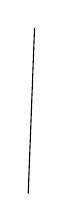
\begin{tikzpicture}\draw (0,0)--(.08,2.1);\end{tikzpicture}}\uline{NB} L'ens des $\widetilde b_i^\omega$ n'est pas stable sous $\tau$ il faudrait donc aussi prendre les $\tau\widetilde b_i^\omega$}
\margin{\figure{\begin{tikzpicture}[scale=.8]
\draw[line width=1.2pt] (0,.35)--(.03,.75);\fill (.68,.24) circle (.7pt);\fill (.74,.33) circle (.7pt);
\end{tikzpicture}}}
On aura
\[
(9)\quad\widetilde b_i^\omega(\varphi_{\omega i}^\omega(g))=\varphi_{\omega'i}^\omega(\rho^{-1}(g))
\qquad\rho^{-1}=\varepsilon_0\sigma_\infty
\qquad\left\{\begin{aligned}
\rho(l_0)&=l_1\\
\rho(l_1)&=l_\infty\\
\rho(l_\infty)&=l_0
\end{aligned}\right.
\]
Les relations 2(b) deviennent
\[
(\unsure{10})\quad\widetilde b_{\omega^2i}\widetilde b_{\omega i}\widetilde b_i=1
\]
\margin{23}
